% Drawing 69/02-6 -- folder 69, batch 02, archive page 31 (PDF page 32).
% Transcription: à gauche du texte, un hexagone de sommets numérotés 1 à 6 (2 et 1 en haut, 3 à gauche, 6 à droite, 4 et 5 en bas), avec toutes ses diagonales ; les côtés 12, 34, 56 sont épaissis à l'encre, les côtés 23, 45, 61 soulignés d'un trait ondulé
% Kind: hexagon with all its diagonals (K6). Method 3 (encoded, rendered from the data). Status: ok.
% Notes: Hexagon 1..6 (2 and 1 at the top, 3 left, 6 right, 4 and 5 at the bottom) with all diagonals: the complete graph K_6 drawn on a hexagon. Sides 12, 34, 56 thick; sides 23, 45, 61 underlined with a wavy stroke on the page (drawn dashed here). The vertex numbers are small and partly hidden; placed after the transcription. Encoded as a graph: the 15 edges of K_6, with the perfect matching 12, 34, 56 marked.
% Coordinates: 1 unit = 1 mm = 1/100 of the crop width (bbox in page fractions: [0.18, 0.42, 0.3, 0.5]).
% Redrawn by Claude (claude-opus-5-5), issue #73, 2026-11-07; not checked by a human; not compiled (no TeX in the session).
% Rights: reproduces part of the work -- behind RENDER_TRANSCRIPTS, never published by itself.
\documentclass[tikz,border=3pt]{standalone}
\usepackage{amsmath,amssymb}
\usetikzlibrary{patterns,arrows.meta}
\tikzset{pencil/.style={black!45}, struck/.style={black!35}, mark/.style={circle,draw,inner sep=1.3pt}, pt/.style={circle,fill,inner sep=0.9pt}, opt/.style={circle,draw,fill=white,inner sep=1.1pt}}
\begin{document}
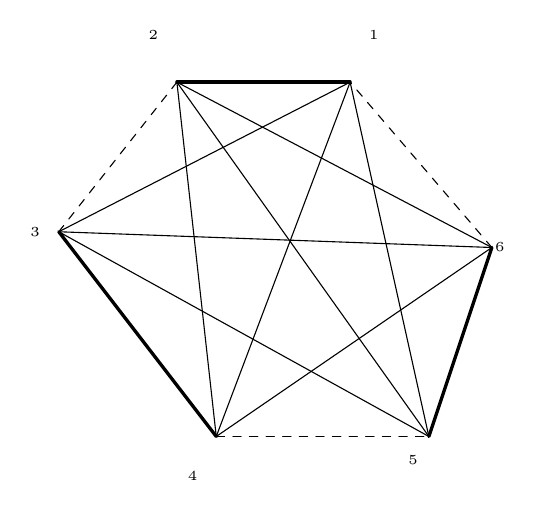
\begin{tikzpicture}[x=1mm,y=1mm,line cap=round,line join=round,font=\scriptsize]
\draw (72,-47) -- (35,-66);
\draw (72,-47) -- (55,-92);
\draw (72,-47) -- (82,-92);
\draw (50,-47) -- (55,-92);
\draw (50,-47) -- (82,-92);
\draw (50,-47) -- (90,-68);
\draw (35,-66) -- (82,-92);
\draw (35,-66) -- (90,-68);
\draw (55,-92) -- (90,-68);
\draw[very thick] (72,-47) -- (50,-47);
\draw[very thick] (35,-66) -- (55,-92);
\draw[very thick] (82,-92) -- (90,-68);
\draw[dashed] (50,-47) -- (35,-66);
\draw[dashed] (55,-92) -- (82,-92);
\draw[dashed] (90,-68) -- (72,-47);
\node[inner sep=1pt] at (47,-41) {\tiny $2$};
\node[inner sep=1pt] at (75,-41) {\tiny $1$};
\node[inner sep=1pt] at (32,-66) {\tiny $3$};
\node[inner sep=1pt] at (91,-68) {\tiny $6$};
\node[inner sep=1pt] at (52,-97) {\tiny $4$};
\node[inner sep=1pt] at (80,-95) {\tiny $5$};
\end{tikzpicture}
\end{document}
